% \documentclass[a4paper]{article}
% \usepackage[ngerman]{babel}
% \usepackage[ansinew]{inputenc}
% \usepackage[top=2.5cm,bottom=1.75cm,right=2cm,left=2.3cm]{geometry}
% \usepackage{floatflt}
% \usepackage{graphicx}\usepackage[colorlinks=true,linkcolor=black,bookmarksnumbered=true,breaklinks=true,pdfstartview=FitH]{hyperref}
% 
% \title{\textbf{Praktikum 4} \\ ~ \\Induktion}
% \author{Michael Kopp}
% \date{27. Februar 2007}
% 
% 
% \begin{document}
% \maketitle


		\section{Magnet im Kupferrohr}

		\subsubsection*{Versuchsbeschreibung:}
In ein 2,5m langes Kupferrohr lässt man einen Magneten fallen. Gleichzeitig lässt man einen gleich schweren Magneten in einem Plastikrohr daneben fallen. Die beiden Rohre sind parallel und stehen senkrecht im Raum. Am Ende der Rohre wird beobachtet, welcher der beiden Magneten die selbse Strecke schneller zurücklegt.		
		
		\subsubsection*{Beobachtungen:}
Der Magnet, der durch das Plastikrohr fiel, ist wesentlich schneller. 
		
		\subsubsection*{Auswertung:}
Ein Körper, der frei im Raum fällt benötigt für die Strecke 2,5m die Zeit \(t_0\). \(t_0\) lässt sich folgendermaßen Berechnen:

\begin{equation}
h = \frac{1}{2} \cdot g \cdot t_0^2 ~~\Rightarrow~~
\frac{2 \cdot h}{g} = t_0^2 ~~\Rightarrow~~
\sqrt{\frac{2 \cdot h}{g}} = t_0 
\end{equation}
Für \(h = 2,5m\) ergibt sich so: \(t_0 = \sqrt{\frac{2 \cdot 2,5}{9,81}} \approx 0,71s\) \marginpar{\(\sqrt{\frac{m}{\frac{m}{s^2}}} = \\ \sqrt{s^2} = s\)}
Die tatsächlich für demn Magneten im Kupferrohr gemessene Zeit \(t_1\) lag aber beträchtlich vom Wert \(t_0\) entfernt -- der Magnet braucht im Kupferrohr deutlich länger.

Das liegt vermutlich daran, dass der Magnet\footnote{dadurch, dass er sich beim Fallen bewegt} in dem Kupferrohr einen Wirbelstrom hervorruft. In diesem Fall liegt also Induktion durch Relativbewegung vor. Aufgrund des \textsc{Lenz}'schen Gesetzes wird in dem Kupferrohr so Induktionsspannung induziert\footnote{und damit ein Strom hervorgerufen}, dass diese ihrer Ursache entgegenwirkt. Um der Ursache entgegenzuwirken, verläuft der Stromfluss so, dass ein Magnetfeld aufgebaut wird, das dem des fallenden Magneten so entgegengerichtet ist, dass dieser abgebremst wird.



		\section{Kraftübertragung auf Alufolie mittels Magnetismus}
		\label{alumag}
	
		\subsubsection*{Versuchsbeschreibung:}
Ein dreifach gefaltetes Stück Alufolie wird auf eine Wasseroberfläche gegeben, sodass es schwimmt. Mit einem Magneten, von dem \emph{ein} Pol auf die Folie gerichtete wird, werden etwa einen Zentimeter über der Folie kreisende Bewegungen ausgeführt.
		
		\subsubsection*{Beobachtungen:}		
Die Alufolie beginnt sich in die Richtung zu drehen, in die man mit dem Magneten kreist. Führt man die Kreisbewegungen dann in die andere Richtung durch, so bremst man die Folie wieder ab.
		
		\subsubsection*{Auswertung:}

Diesen Vorgang kann man durch das \textsc{Lenz}'sche Gesetz erklären. Dadurch dass der Magnet über der Alufolie bewegt wird, wird in der Folie ein Wirbelstrom erzeugt - es handelt sich um Induktion durch \textit{Relativbewegung}\footnote{Die Relativbewegung ist also die \textit{Ursache} der Induktion}.

Dieser Wirbelstrom baut um sich ein Magnetfeld auf. Gemäß dem \textsc{Lenz}\'schen Gesetz baut dieses Magnetfeld sich nun so auf, dass es seiner Ursache entgegenwirkt. Die Ursache der Induktion ist in diesem Fall wie oben ausgeführt eine Relativbewegung. Das Magnetfeld des Wirbelstroms wird nun so entstehtn, dass es dieser Relativbewegung entgegenwirkt, also die Relativbewegung beendet. 

Dies wird erreicht, indem die Alufolie sich möglichst genau so schnell wie der Magnet bewegt, da sich ohne Geschwindigkeitsdifferenz zwischen den beiden Bewegungen keine weitere Induktion ergibt.

Beendet man die Bewegung des Magneten oder ändert gar seine Richtung, so gilt erneut das \textsc{Lenz}'sche Gesetz, das wiederum dafür sorgt, diese 'neue' Relativbewegung aufzuheben.





%Da Aluminium nicht zu den Stoffen gehören, die von sich aus magnetisierbar sind\footnote{wie Eisen, Nickel oder Cobalt}, wird wohl ein Strom in der Alufolie induziert. Es liegt wieder Induktion durch Relativbewegung vor. Die Elektronen werden durch die \textsc{Lorentz}kraft senkrecht zu der Richtung abgelenkt, in die der Magnet bewegt wird\footnote{nach der Linken-Hand-Regel}. In Graphik \ref{vec01} auf Seite \pageref{vec01} sind die Vektoren dieser Vorgänge dargestellt. Daraus ist ersichtlich, dass die Kraft \(F_R\) die Alufolie im Prinzip unter dem Magneten wegdrückt, weil sie entgegen der Bewegungsrichtung des Magneten auf diesen einwirkt. 
%
%Je schneller man mit dem Magneten kreist, desto stärker ist diese Kraft und desto schneller kann man die Alufolie auch antreiben. Wechselt man die Rotationsrichtung, so ändern sich alle Vektoren schlichtweg in ihre  (auf vorher bezogene) Gegenrichtung. Durch die \textsc{Lorentz}kraft werden die Elektronen in ihrer Kreisbahn zuerst ausgebremst und dann auf Gegenkurs gebracht. Dadurch, dass die Kraft \(F_R\) nun wieder entgegen der Bewegung des Magneten steht, drückt diese Kraft die Alufolie und den Magneten voneinander weg. Da die Kraft \(F_R\) so schwach\footnote{bozogen auf die (träge) Masse und relativ große Reibung der Alufolie} ist, braucht die beschleunigende bzw. bremsende Wirkung eine Weile, um den Bewegungszustand der Alufolie zu ändern.
%
%Wichtig ist dabei auch, dass stets die Elektronen die Kräfte erfahren. Die Kraft \(F_R\) entsteht dadurch, dass die Elektronen im Kreis fließen, also ein Wirbelstrom entsteht und dieser ein Magnetfeld aufbaut, das gemäß dem \textsc{Lenz}'schen Gesetz dem Magnetfeld des Stabmagneten entgegengerichtet ist. \(F_R\) ist also die Kraft, resultierend aus der Abstoßung zweier gleichnamiger Magnetpole\footnote{bzw. ihrer Felder}.
%
%
%
%\begin{figure}[ph]
%\centering
%\includegraphics[height=4.5cm]{a.pdf}
%\caption{Die Vektoren von Kraft und Geschwindigkeit zu Aufgabe \ref{alumag}. \(F_M\) steht für die Kraft, mit der man den Magneten bewegt, \(F_L\) steht für die Kraft, mit der die Elektronen abgelenkt werden, \(v_{EL}\) steht für die Geschwindigkeit, mit der sich die Elektronen bewegen und \(F_R\) steht für die Kraft, die der Induktionsstrom auf den Magneten auswirkt.}
%\label{vec01}
%\end{figure}


		\section{Wirbelstrombremse}
		\label{wistrobre}
		
		\subsubsection*{Versuchsbeschreibung:}
Ein Motor treibt eine Scheibe an. Diese dreht sich an einer Stelle durch das (starke) Magnetfeld eines Dauermagneten. An der Scheibe ist an einer Stelle ein Fähnchen montiert. Es dient zur Drehfrequenzbestimmung, da eine Lichtschranke so angebracht ist, dass das Fähnchen bei jeder Umdrehung die Lichtschranke passieren muss. Bei dem Motor wird die Spannung kontrolliert erhöht und dazu die Stromstärke gemessen.
		
		\subsubsection*{Beobachtungen:}		
Die Wirbelstrombremse funktioniert nur dann, wenn man Scheiben aus Metall verwendet. Für eine Kupferscheibe ergeben sich Messergebnisse, wie sie in Tabelle \ref{tabkup1} auf Seite \pageref{tabkup1} zusammengestellt sind. In Tabelle \ref{tabmat1} auf Seite \pageref{tabmat1} sind Ergebnisse zu anderen Materealien zusammengestellt.

Aus den Schaubildern \ref{abbkup1a} auf Seite \pageref{abbkup1a} und \ref{verschmat} auf Seite \pageref{verschmat} ist klar ersichtlich, dass der Zusammenhang zwischen der Drehgeschwindigkeit der Scheibe und der Stromstärke linear ist. Trägt man die Ausgleichsgeraden aller Messungen in ein gemeinsames Schaubild ein, so erhält man daraus Abbildung \ref{ausglger} auf Seite \pageref{ausglger}.

\begin{table}[h]
\centering
\begin{tabular}{c c c | c c c | c c c}
\multicolumn{3}{c}{\textbf{Kupfer I}} & \multicolumn{3}{c}{\textbf{Kupfer II}} & \multicolumn{3}{c}{\textbf{Kupfer III}} \\
\textbf{\textit{U [V]}}	&	\textbf{\textit{f [\(s^{-1}\)]}}  &	\textbf{\textit{I [A]}} & \textbf{\textit{U [V]}}	&	\textbf{\textit{f [\(s^{-1}\)]}}  &	\textbf{\textit{I [A]}} & \textbf{\textit{U [V]}}	&	\textbf{\textit{f [\(s^{-1}\)]}}  &	\textbf{\textit{I [A]}} \\
\hline
2	&	4,8	&	0,08	&	2	&	4,6	&	0,06	&	2	&	4,8	&	0,06 \\
3	&	8,2	&	0,11	&	4	&	9,5	&	0,13	&	4	&	9,9	&	0,13 \\
4	&	11,4	&	0,14	&	6	&	13,9	&	0,20	&	6	&	14,6	&	0,20 \\
5	&	14,5	&	0,18	&	8	&	18,8	&	0,27	&	8	&	19,6	&	0,26 \\
6	&	17,5	&	0,21	&		&		&		&	10	&	24,9	&	0,34 \\
7	&	20,5	&	0,24	&		&		&		&		&		&	\\
8	&	23,5	&	0,27	&		&		&		&		&		&	\\
9	&	26,3	&	0,30	&		&		&		&		&		&	\\
10	&	29,0	&	0,32	&		&		&		&		&		&	\\
\end{tabular}
\caption{Ergebnisse von drei Messungen des Versuches aus Aufgabe \ref{wistrobre} mit einer Kupferscheibe}
\label{tabkup1}
\end{table}


\begin{table}[h]
\centering
\begin{tabular}{c c c | c c c}
\multicolumn{3}{c}{\textbf{Aluminium}} & \multicolumn{3}{c}{\textbf{Kunststoff}} \\
\textbf{\textit{U [V]}}	&	\textbf{\textit{f [\(s^{-1}\)]}}  &	\textbf{\textit{I [A]}} & \textbf{\textit{U [V]}}	&	\textbf{\textit{f [\(s^{-1}\)]}}  &	\textbf{\textit{I [A]}} \\
\hline
2,00	&	5,80	&	0,05	&	2,00	&	9,60	&	0,02 \\
4,00	&	11,20	&	0,10	&	4,00	&	20,80	&	0,02 \\
6,00	&	17,10	&	0,16	&	6,00	&	30,90	&	0,03 \\
8,00	&	23,50	&	0,22	&	8,00	&	41,10	&	0,04 \\
10,00	&	29,20	&	0,28	&	10,00	&	51,20	&	0,05 \\
\end{tabular}
\caption{Ergebnisse zu Messungen mit anderen Materealien aus Aufgabe \ref{wistrobre}}
\label{tabmat1}
\end{table}




\begin{figure}[htb]
	\centering
		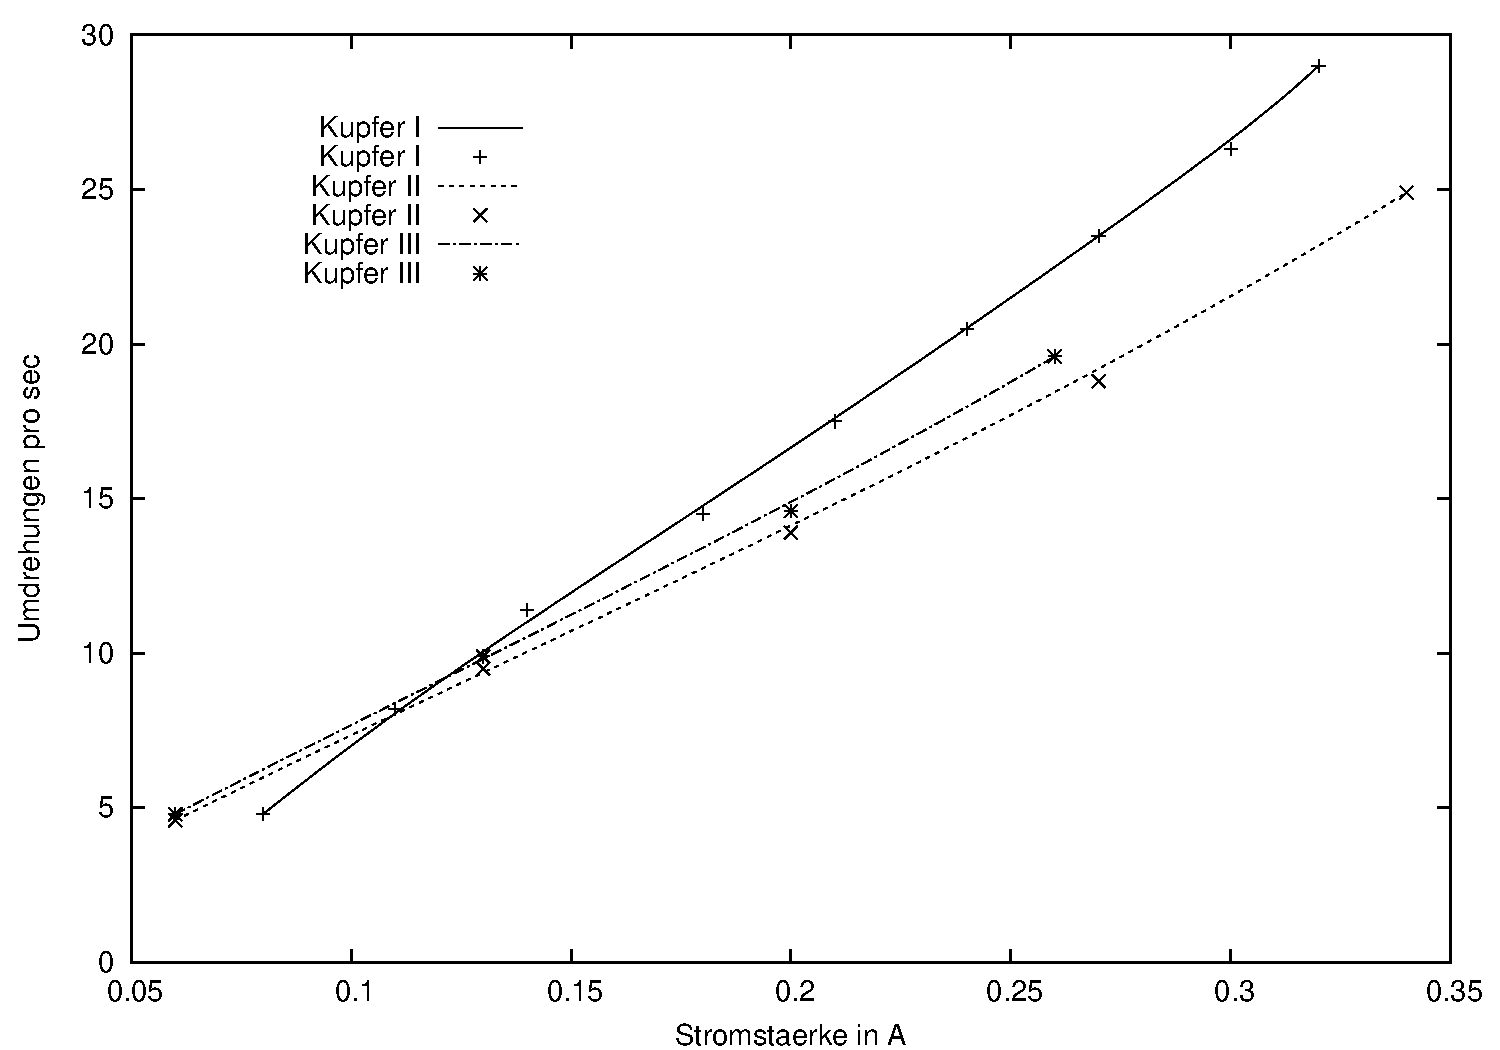
\includegraphics[width=0.95\textwidth]{praktika/mat_praktika/b2}
	\caption{Ergebnisse der Messung des Versuches aus Aufgabe \ref{wistrobre} mit einer Kupferscheibe. In dem Schaubild sind die Daten von drei verschiedenen Messungen enthalten -- Kupfer I bis III --, jeweils mit Datenpunkten und einer Ausgleichskurve.}
	\label{abbkup1a}
\end{figure}


\begin{figure}[htb]
	\centering
		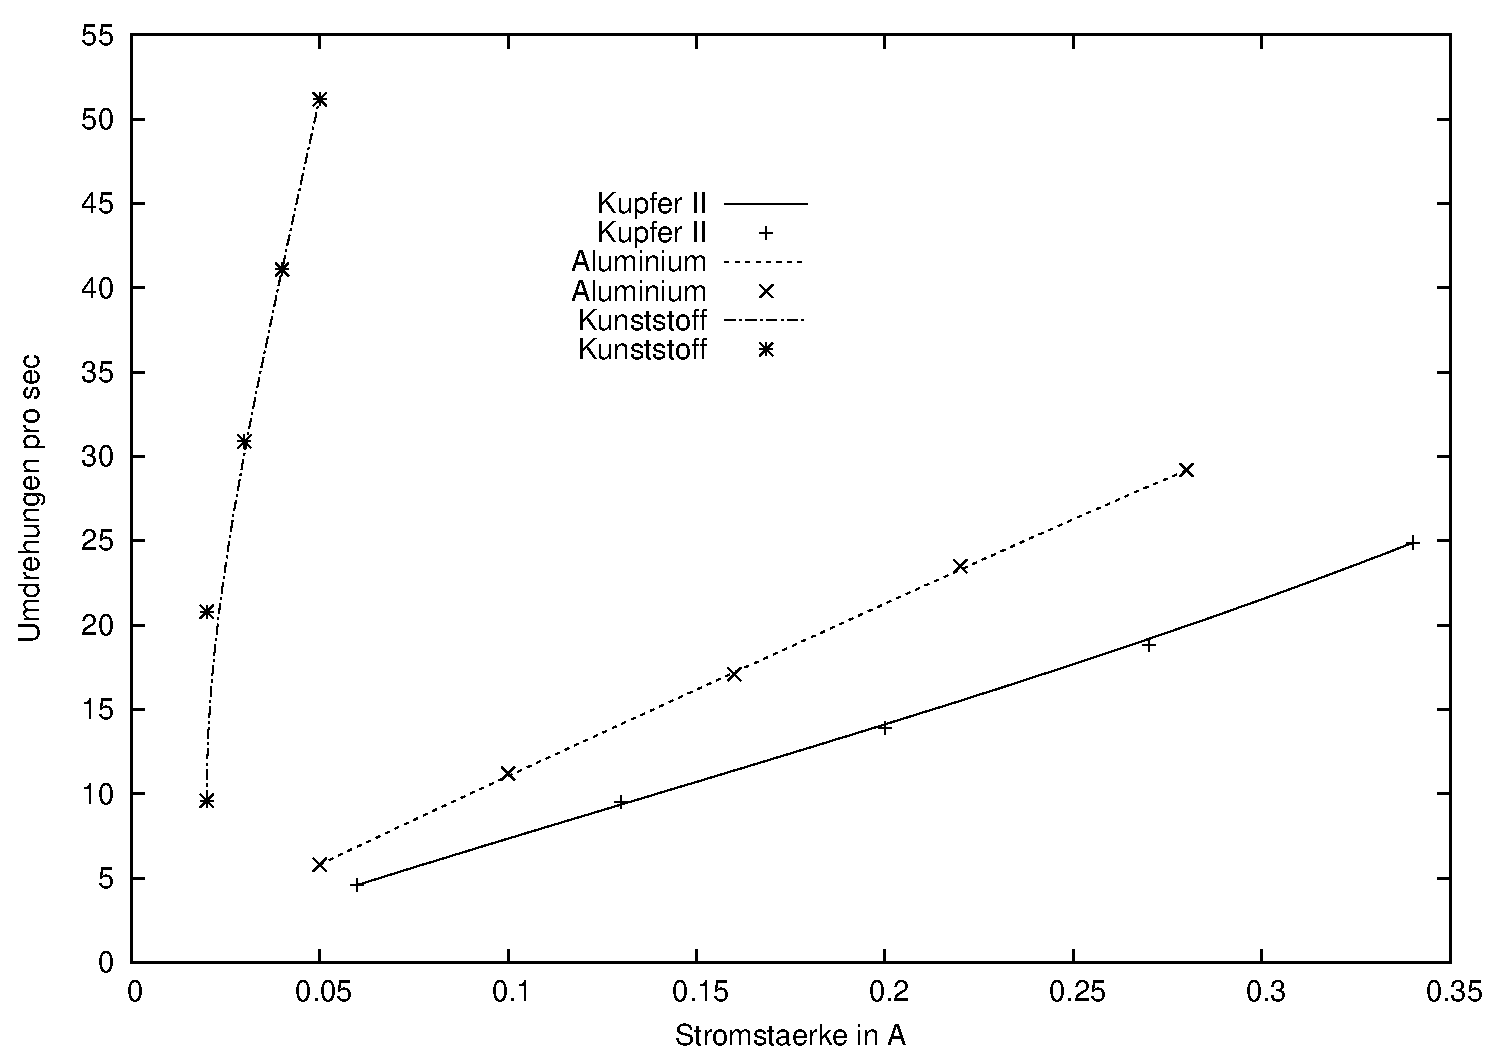
\includegraphics[width=0.95\textwidth]{praktika/mat_praktika/p1db1}
	\caption{Ergebnisse der Messung verschiedener Materealien des Versuches aus Aufgabe \ref{wistrobre} mit Ausgleichskurven.}
\label{verschmat}
\end{figure}


\begin{figure}[htb]
	\centering
		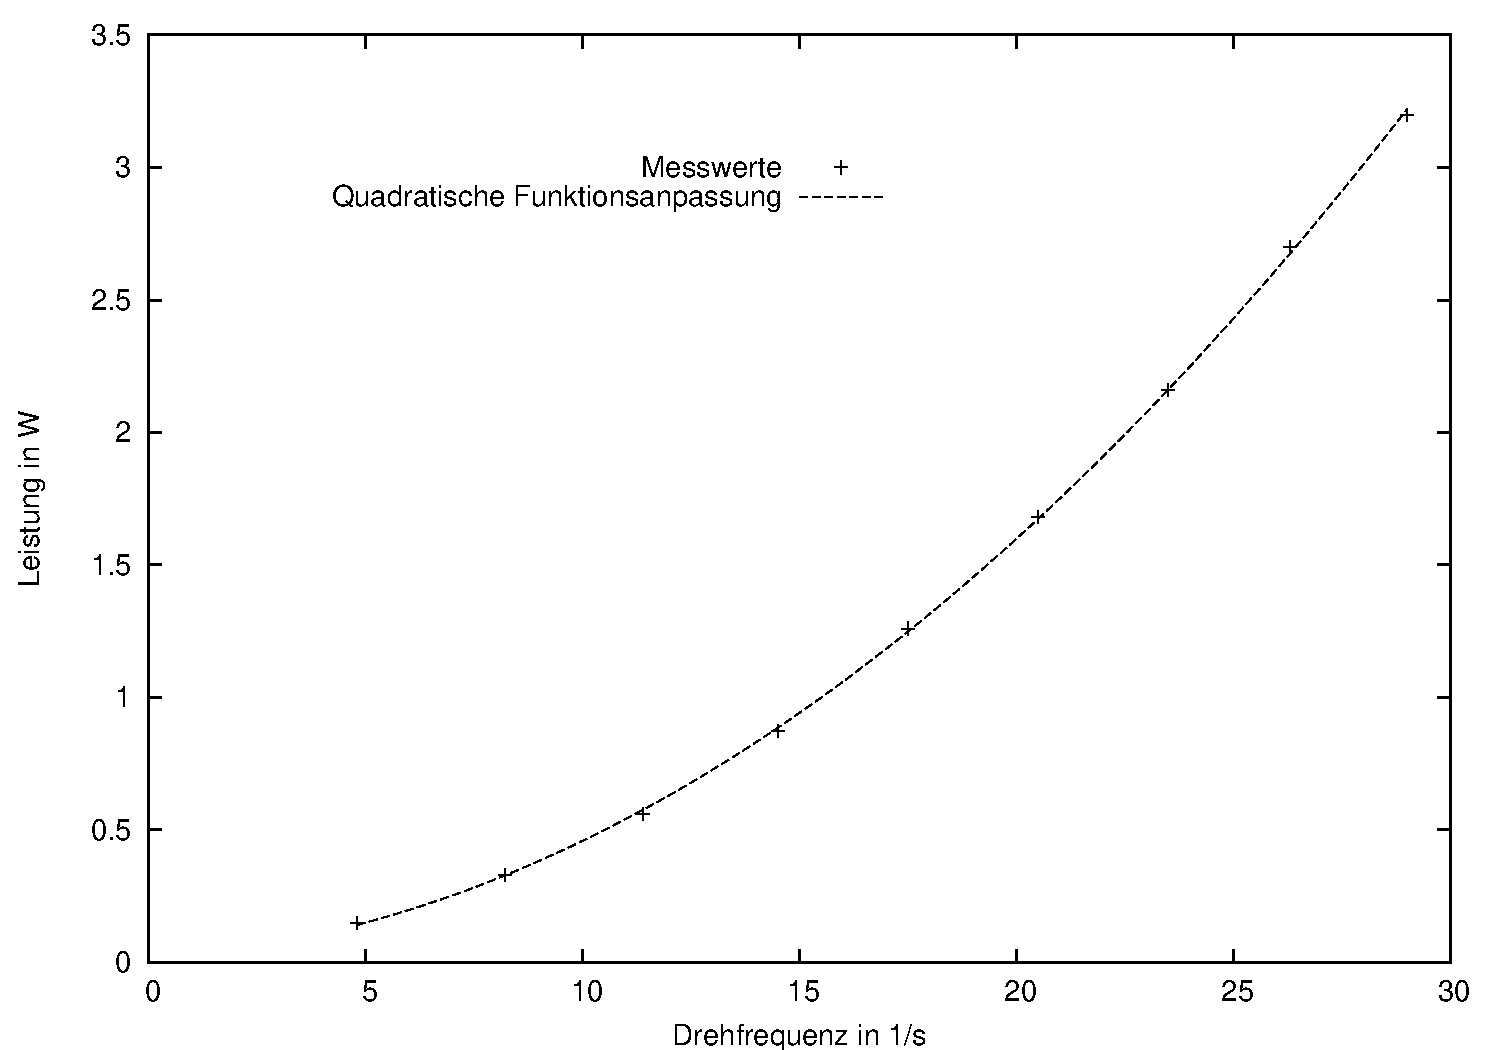
\includegraphics[width=0.95\textwidth]{praktika/mat_praktika/c}
	\caption{Ergebnisse der Messung Kupfer I des Versuches aus Aufgabe \ref{wistrobre} mit einer Kupferscheibe - mit quadratischer Regression}
	\label{abbkup1b}
\end{figure}


\begin{figure}[htb]
	\centering
		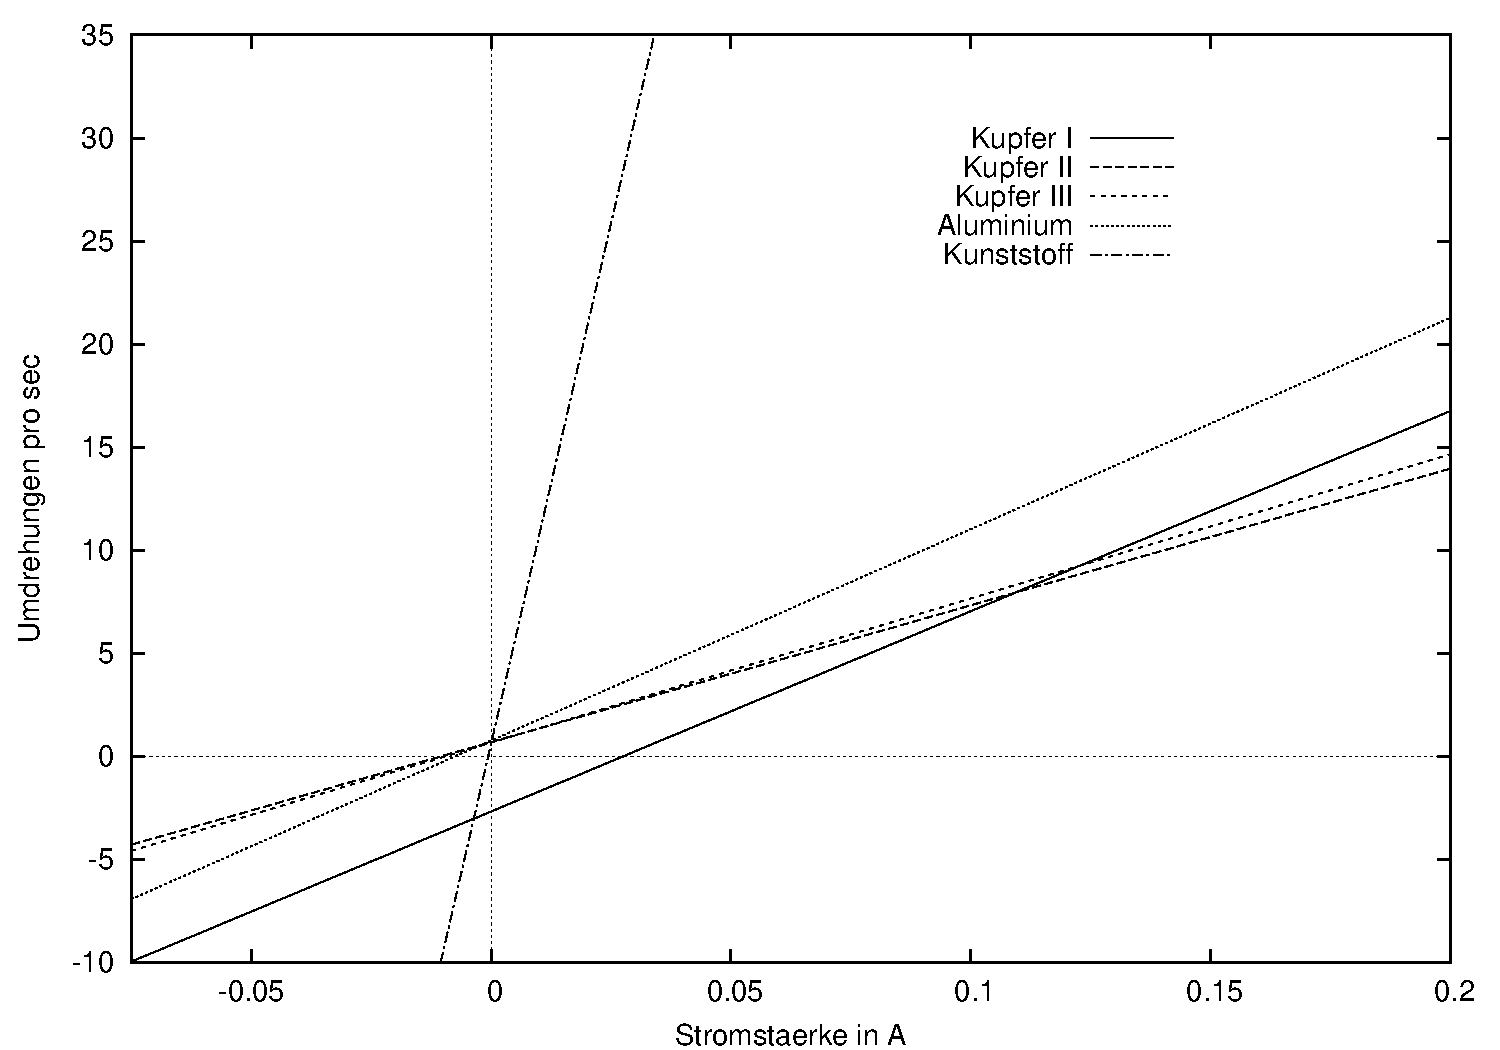
\includegraphics[width=0.9\textwidth]{praktika/mat_praktika/sa1}
	\caption{Die Ausgleichsgeraden aller Messungen zu Aufgabe \ref{wistrobre} in einem Schaubild eingetragen.}
	\label{ausglger}
\end{figure}





		\subsubsection*{Auswertung:}
In Abbildung \ref{abbkup1a} auf Seite \pageref{abbkup1a} ist die Drehfrequenz in Abhängigkeit zur Stromstärke aufgetragen. Es wurde eine Ausgleichsgerade eingetragen, die mit dem Messwerten äußerst gut übereinstimmt. Es liegt also nahe, dass Drehfrequenz und Stromstärke zueinander proportional sind. Es gilt also:
\begin{equation}
f \sim I
\label{eqsimfi}
\end{equation}
In Abbildung \ref{abbkup1b} auf Seite \pageref{abbkup1b} sind dann Leistung und Drehfrequenz gegeneinander aufgetragen. Dabei wird deutlich, dass die zur Drehung benötigte Leistung bei steigenden Drehfrequenzen quadratisch ansteigt. Es gilt also: 
\begin{equation}
P \sim f^2
\label{eqsimfp}
\end{equation}
Verbindet man \ref{eqsimfi} und \ref{eqsimfp}, so erhält man
\begin{equation}
P \sim I^2
\end{equation}
Das ist aber einfach erklärbar\footnote{Da im Motor der Strom durch Spulen fließt - also gewickeltem Draht - kann man nährungsweise davon ausgehen, dass es sich hierbei um einen \textsc{Ohm}'schen Widerstand handelt. Da der Motor mit Gleichstrom betrieben wird, sind Induktionsvorgänge vernachlässigbar.}, da ja 
\begin{equation}
P = I \cdot U ~~  \textnormal{und} ~~ U = I \cdot R ~~ \textnormal{und somit} ~~ P = I^2 \cdot R
\label{eq:ohmges}
\end{equation}
Aus Abbildung \ref{ausglger} auf Seite \pageref{ausglger} ist darüber hinaus ersichtlich, dass die Ausgleichsgeraden Ursprungsgeraden sind - nur eine widersetzt sich diesem Trend. Es könnte nun einerseits sein, dass hier bei besonders niedriger Umdrehungszahl die Reibung äußerst groß ist und die Kurve deshalb so nach unten \textit{absackt}. Wahrscheinlicher ist jedoch, dass mit den Messgeräten etwas nicht stimmt (da die Werte auf eine dermaßen exakten Linie liegen).

Daraus, dass Kurve des Kunststoffes wesentlich steiler ist, kann man ablesen, dass er für die selbe Drehfrequenz weniger Energie braucht. Dass dies auf das geringere Gewicht der Scheibe zurückzufürhen ist, ist unwahrscheinlich. Da eine Messung über 10 sec dauert, hatte der Motor -- wenn er eine schwerere und damit trägere Kupferscheibe antreibt -- genug Zeit, auch mit geringerer Beschleunigung seine maximale Geschwindigkeit zu erreichen. Es ist also davon auszugehen, dass die gemessenen Drehfrequenzen maximal für die Leistung des Motors ist und dabei nicht von der trägen Masse der Scheiben abhängt. 

Viel wahrscheinlicher ist, dass die Kupfer- und Aluminiumscheiben von der Wirbelstrombremse beeinflusst werden -- im Gegensatz zur Plastikscheibe. Der Motor muss somit, wenn er eine Kupferscheibe antreibt, immer gegen die bremsende Kraft der Wirbelstrombremse antreiben.

\clearpage
		\section{Strom- und Spannungsverlauf bei Selbstinduktion}
		\label{seind}
		
		\subsubsection*{Versuchsbeschreibung:}
Es wird ein Stromkreis gemäß Abbildung \ref{schzk} auf Seite \pageref{schzk} aufgebaut. Wenn der Schalter \(S_1\) geschlossen ist, so fließt Strom parallel - einerseits durch die Spule und \(R_2\), andererseits durch \(R_1\). Wird der Schalter \(S_1\) geöffnet, so fließt ein Induktionsstrom dem Verlauf der gestrichelten Pfeile nach, also in Reihe durch \(R_1\), \(R_2\) und die Spule. 

\begin{figure}[hp]
\centering
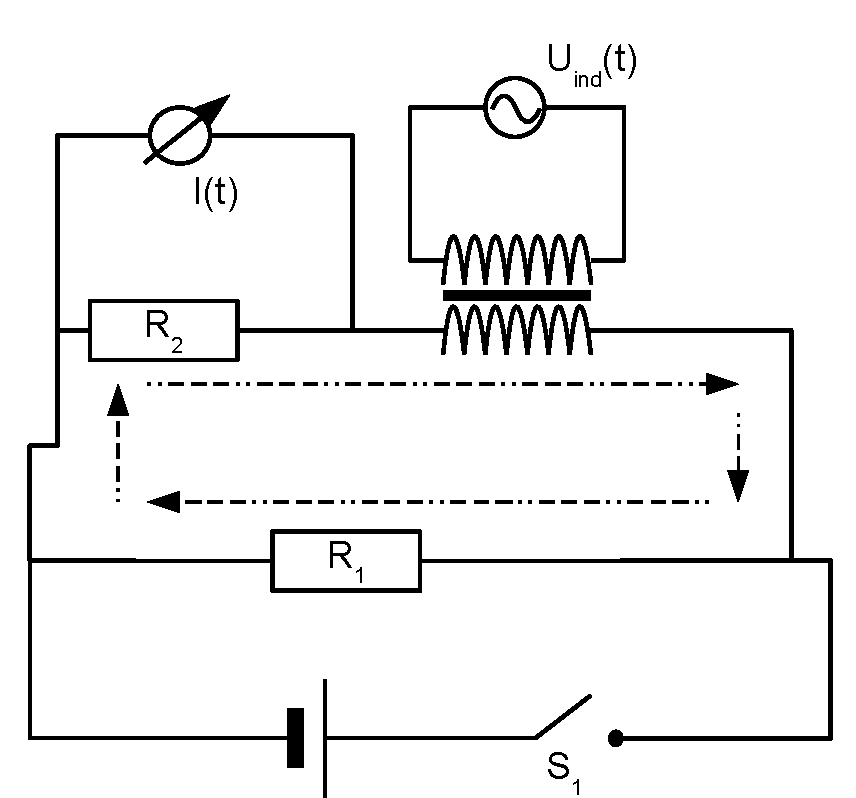
\includegraphics[width=0.3\textwidth]{praktika/mat_praktika/sz1}
\caption{Schaltdkizze zum Versuchsaufbau von Aufgabe \ref{seind}: \(R_1\) und \(R_2\) haben jeweils \(R_n = 220 \Omega\), die beiden Spulen haben jeweils \(n = 800\) Windungen, die Spannungsquelle liefert \(U_0 = 10V\) und der Schalter \(S_1\) ist ein \textit{Doppelreedrelais}, das mit der Frequenz \(f = 50 Hz\) umschaltet.}
\label{schzk}
\end{figure}

		

An \(R_2\) wird die Spannung gemessen. Da es sich bei \(R_2\) um einen Ohmschen Widerstand handelt, ist \(U(t) \sim I(t)\) (\(\rightarrow\) Gleichung \ref{eq:ohmges}). Deshalb ist es möglich, an \(R_2\) die Stromstärke \(I(t)\) abzulesen, da sie ja zu der eigentlich abgelesenen Spannung proportional ist.

An die zweite Spule, die mit der ersten durch einen gemeinsamen Eisenkern vebunden ist, wird ein Oszilloskop angeschlossen. Wird in der ersten Spule eine Induktionsspannung \(U_{ind}(t)\) induziert, so ist dazu ein sich änderndes Magnetfeld \(\dot{B} \neq 0\) nötig. Dieses sich ändernde Magnetfeld hat über den gemeinsamen Eisenkern auch in der zweiten Spule Auswirkungen, nämlich wird dort gemäß \(U_{ind} = n \cdot A \cdot \dot{B}\) die selbe Induktionsspannung wie in der ersten Spule induziert.

Somit kann man an \(R_2\) und der zweiten Spule \(I(t)\) bzw. \(U_{ind}(t)\) bestimmen.


		\subsubsection*{Beobachtungen:}
In Abbildung \ref{oszbu} auf Seite \pageref{oszbu} ist der Verlauf der Induktionsspannung dargestellt. In Abbildung \ref{oszbi} ist die Spannung dargestellt, die am Widerstand \(R_2\) abfällt. Vergleicht man die beiden Spannungsverläufe miteinander, so fällt auf, dass die Induktionsspannung	genau dann einen extremen \textit{Peak} nach oben macht, wenn der Strom gerade seinen Höchstpunkt erreicht hat und gerade am Absinken ist. Wenn der Strom gerade wieder ansteigt, so ist die Induktionsspannung stark negativ.


		\subsubsection*{Auswertung:}
Diese Phänomene sind duch \textit{Induktion} erklärbar. Wenn nämlich der Strom eingeschaltet wird, also in Schaubild \ref{oszbi} die Funktion sich gerade von der Zeitachse entfernt, ist die Änderung des Stromes \(\dot{I}(t)\) äußerst groß, da sich die Spannung ja von "`überhaupt kein Wert"' auf "`einen positiven Wert"' ändert. Nach 
\begin{equation}
	U_{ind}(t_n) = - L \cdot \dot{I}(t_n)
	 \label{lenz}
\end{equation}
ist die Induktionsspannung hier also stark negativ. Mit dem \textsc{Lenz}'schen Gesetz in Einklang ist diese Induktionsspannung also ihrer Ursache entgegengesetzt und "`\textit{fängt}"' die Veränderung der Stromstärke ab. Der Stromverlauf ist deshalb an dieser Stelle auch kurvenförmig. Ohne die entgegengerichtete Induktionsspannung hätte der Strom sein Maximum praktisch sofort erreicht. So nährt er sich seinem Maximum nur asymptotisch an.

Je mehr Zeit innerhalb einer halben Periode verstreicht, desto näher kommt der ausgebremste Strom seinem Maximum, aber immernoch ist eine gegenläufige Spannung da, die ihn dezimiert. Da er konsequent dezimiert wird, wird \(\dot{I}(t_N)\) auch kleiner, da ja ständig die wachstumsschwächende Induktionsspannung auf den Strom einwirkt.

Wenn der Strom dann wieder abgeschaltet wird, also von seinem Maximum abfällt (vgl Abbildung \ref{oszbi}), ist in Schaubild \ref{oszbu} ein noch größerer Peak entstanden, dier diesmal nach oben zeigt, also auch eine große positive Spannung hinweist. \(\dot{I}(t_n)\) ist an dieser Stelle stark negativ, weil der Strom sich von einem nahezu konstannten Wert "`\textit{erstmalig}"' abbewegt. Nach Gleichung \ref{lenz} sorgt diese Spannung nun dafür, dass der Stromstärkenabfall abgefangen wird, also nicht so drastisch aussieht.


\begin{figure}[h]
\centering
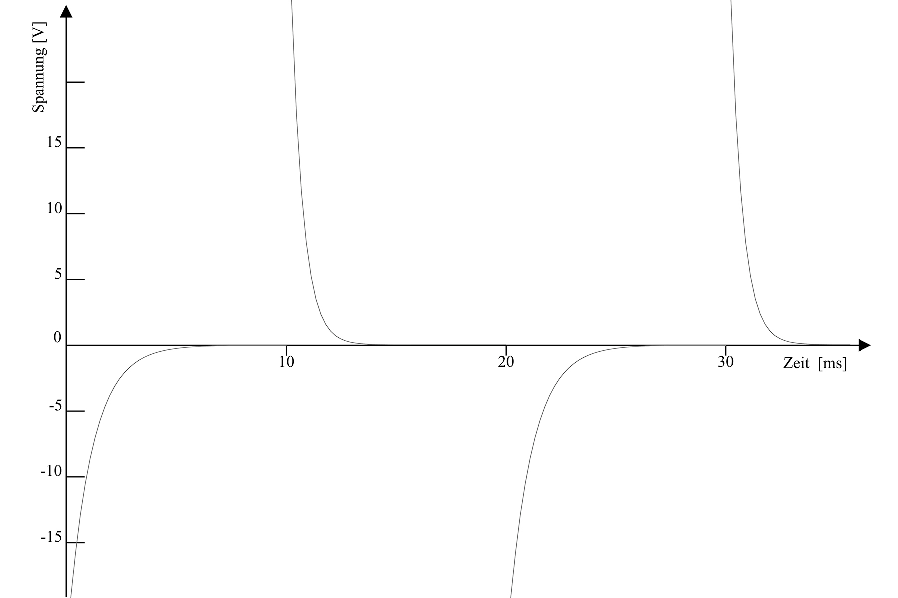
\includegraphics[width=0.85\textwidth]{praktika/mat_praktika/f1c}
\caption{Im Oszilloskop sieht der Spannungsverlauf von \(U_{ind}(t)\) so aus.}
\label{oszbu}
\end{figure}

\begin{figure}[h]
\centering
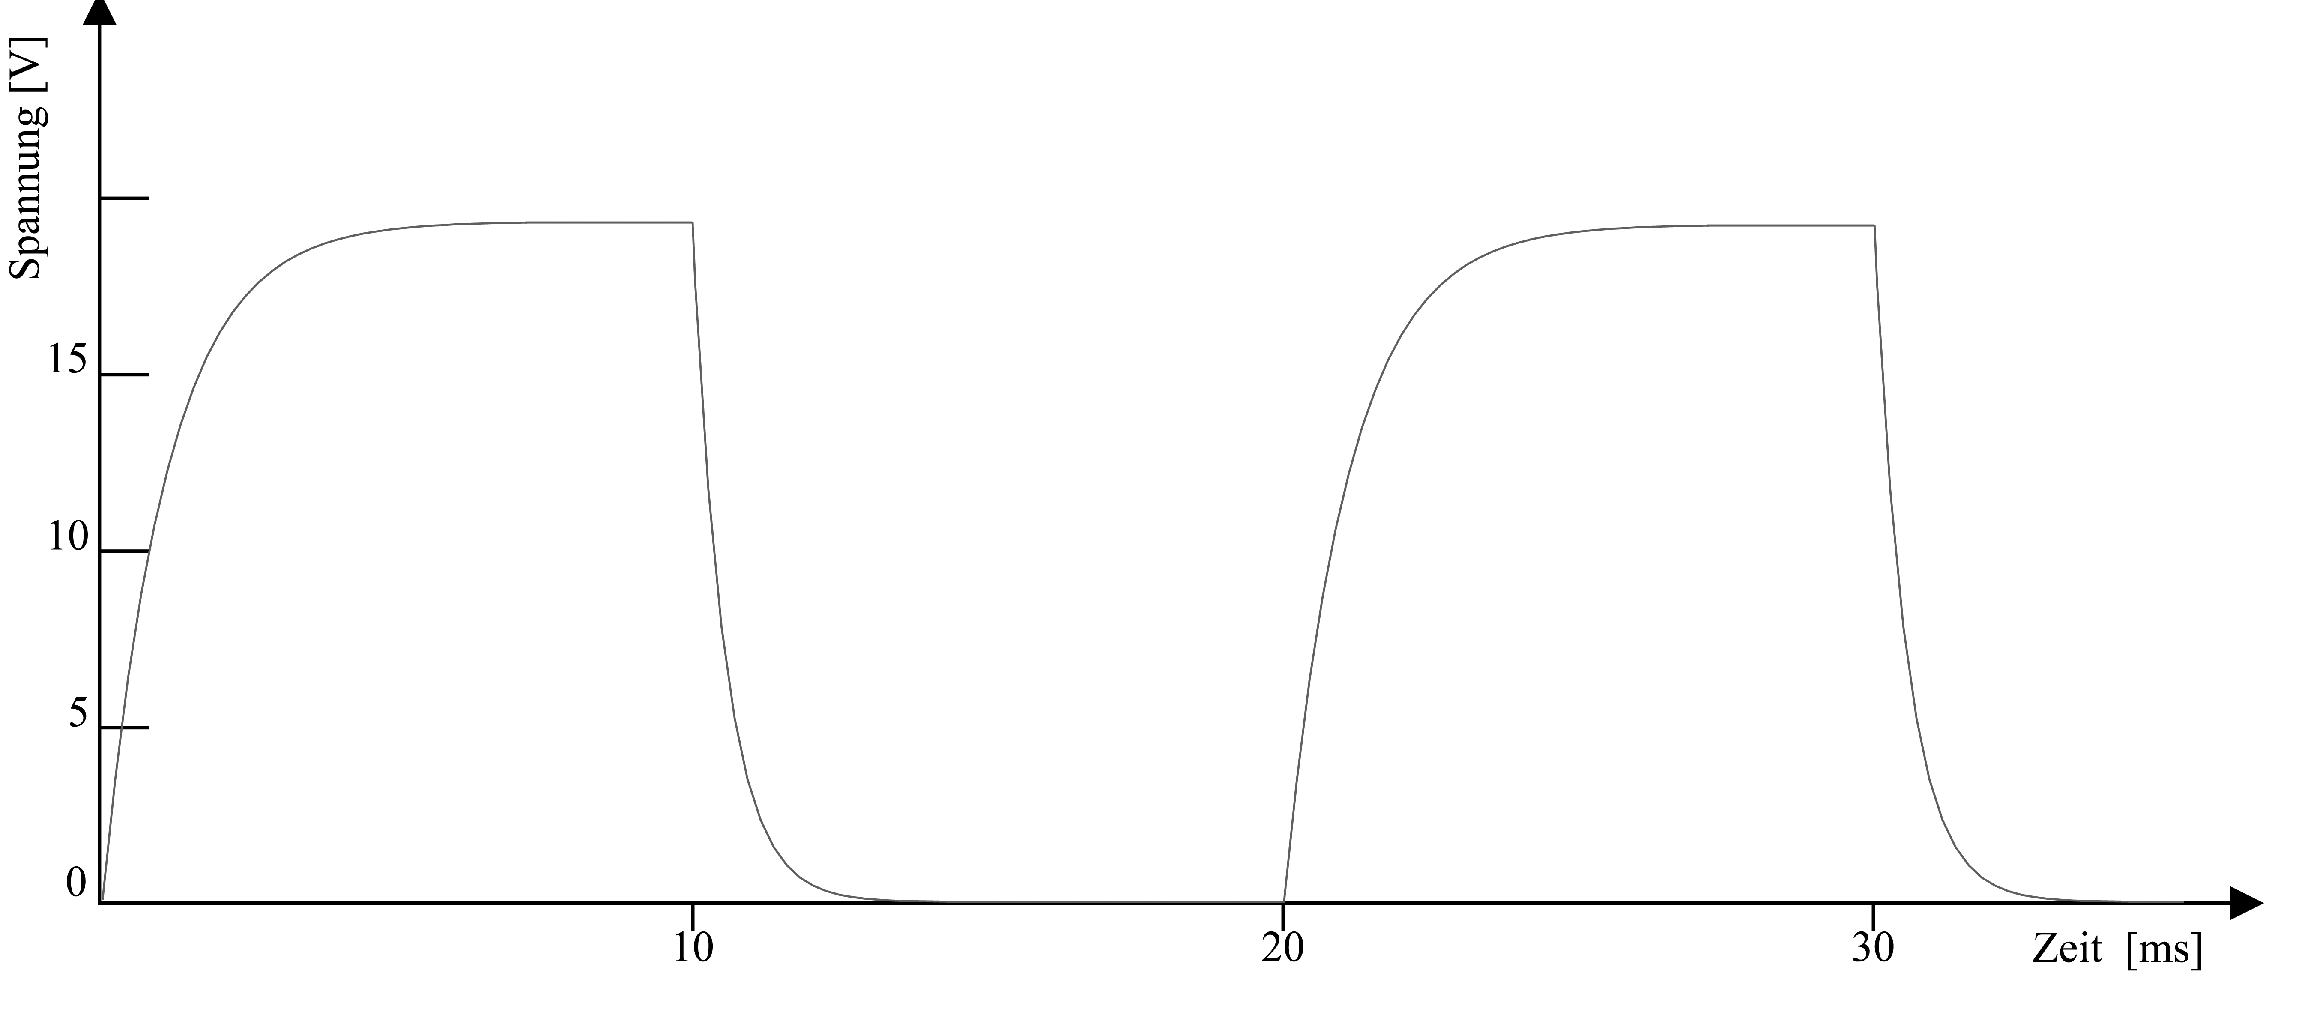
\includegraphics[width=0.85\textwidth]{praktika/mat_praktika/g1a}
\caption{Der Spannungsverlauf von \(U_{R_{2}}(t)\) dient zur bestimmung der Stromstäkre \(I(t)\)}
\label{oszbi}
\end{figure}

		





%\end{document}
